%!TEX root = ../../book_ML.tex
\chapter{Máy vector hỗ trợ hạt nhân}
% \chapter{Kernel support vector machine}
\label{cha:kernelsvm}
\section{Giới thiệu}
% \index{SVM hạt nhân -- kernel SVM}
 
Có một sự tương đồng thú vị giữa hai nhóm thuật toán phân loại phổ biến nhất: mạng neuron và máy vector hỗ trợ. Chúng đều bắt đầu từ bài toán phân loại nhị phân 
với hai lớp dữ liệu tách biệt tuyến tính, phát triển tiếp cho trường hợp hai lớp gần tách biệt tuyến tính, tới các bài toán phân loại đa lớp và cuối cùng là các
bài toán với các lớp dữ liệu hoàn toàn không tách biệt tuyến tính. Sự tương đồng này 
có thể thấy trong Bảng \ref{tab:21_1}.
 
 
\begin{table}[h!]
\centering
\caption{Sự tương đồng giữa mạng neuron và máy vector hỗ trợ}
\label{tab:21_1}
\def\arraystretch{1.5}
\setlength\tabcolsep{5pt}
\begin{tabular}{|l|l|l|}
\hline
\textbf{Mạng neuron} & \textbf{Máy vector hỗ trợ}& \textbf{Tính chất chung} \\ \hline
PLA                 &  SVM lề cứng        & Hai lớp tách biệt tuyến tính             \\ \hline  
Hồi quy logistic & SVM lề mềm    & Hai lớp gần tách biệt tuyến tính        \\ \hline 
Hồi quy softmax     & SVM đa lớp   & Nhiều lớp dữ liệu, ranh giới tuyến tính              \\ \hline 
Mạng neuron đa tầng & SVM hạt nhân         & Bài toán phân loại hai lớp không tách biệt tuyến tính \\ \hline
\end{tabular}
\end{table}
 
Trong chương này, chúng ta cùng thảo luận về \textit{SVM hạt nhân} (kernel SVM) cho bài toán phân loại dữ liệu không tách biệt tuyến tính. Bài toán phân loại đa lớp sử dụng ý tưởng SVM sẽ được thảo luận trong chương tiếp theo.
\index{SVM hạt nhân -- kernel SVM}
\index{mô hình hạt nhân -- kernel model}

Ý tưởng cơ bản của SVM hạt nhân và các \textit{mô hình hạt nhân} (kernel model) nói chung là tìm một phép biến đổi dữ liệu không tách biệt tuyến tính ở một không gian thành dữ liệu (gần) tách biệt tuyến tính trong một không gian mới. Nếu có thể thực hiện điều này, bài toán phân loại sẽ
được giải quyết bằng SVM lề cứng/mềm.



% ******************************************************************************
\begin{figure}[t]
    \begin{subfigure}{0.325\textwidth}
    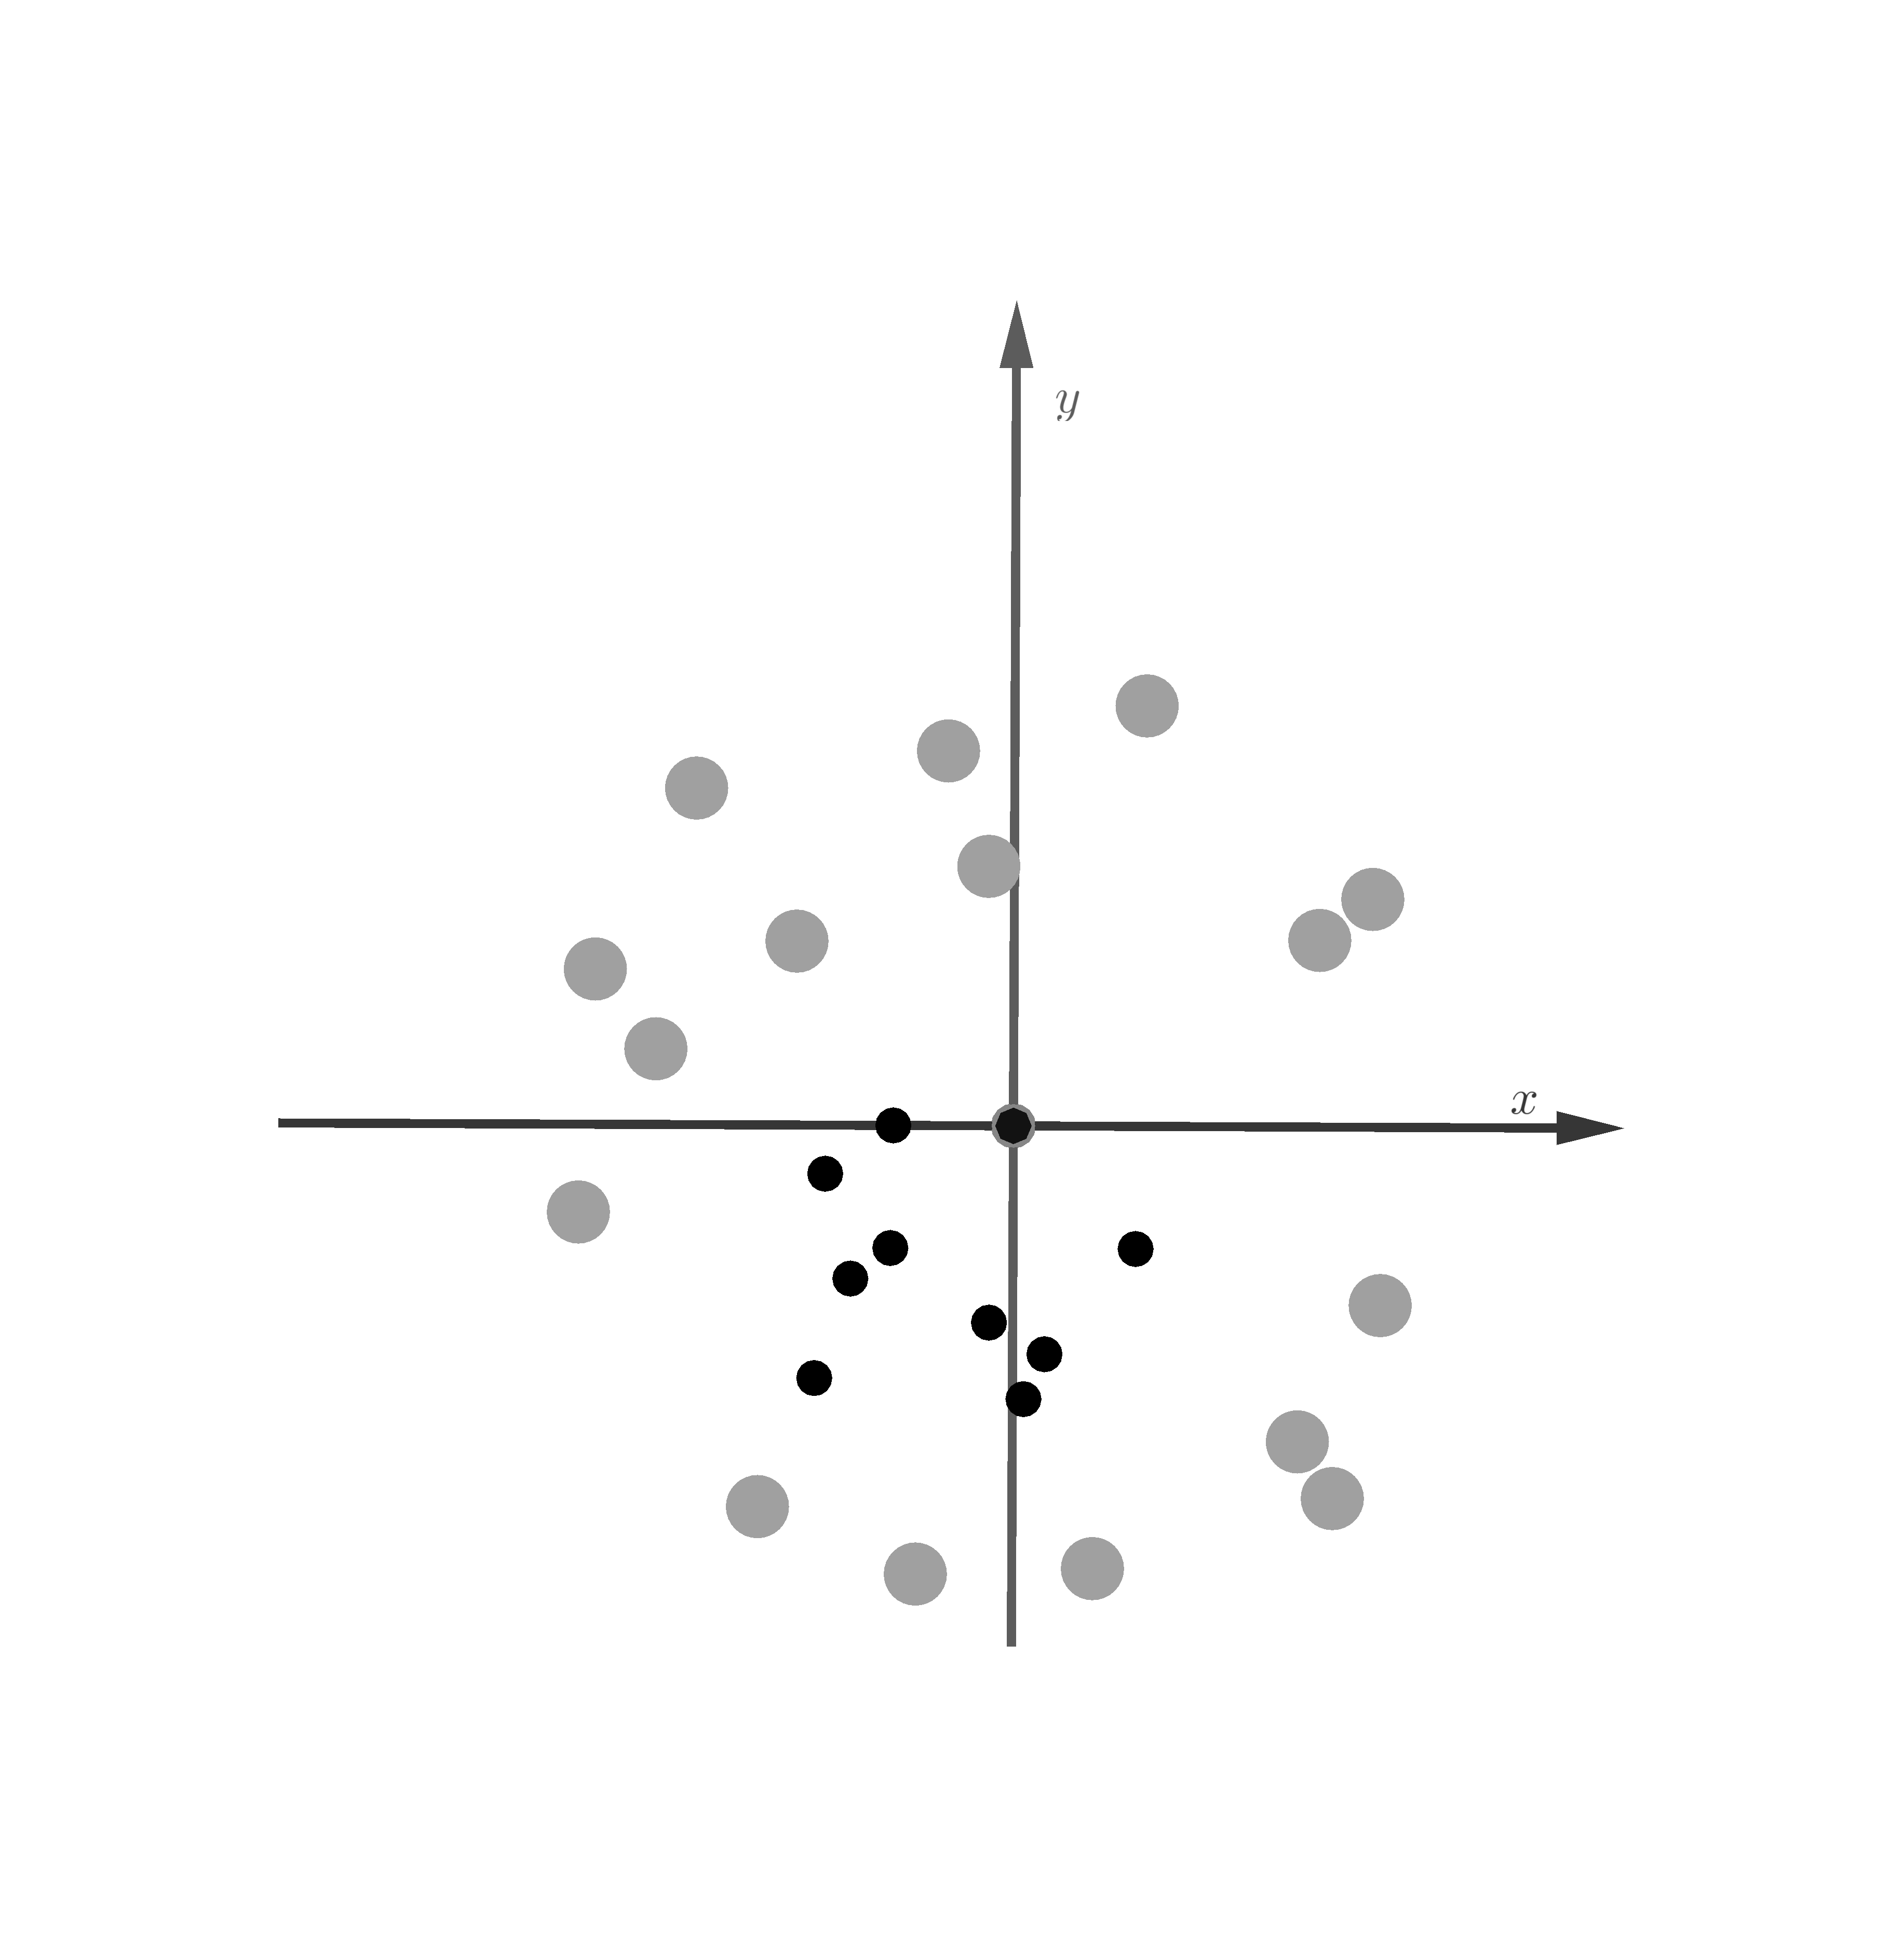
\includegraphics[width=\linewidth]{Chapters/09_SupportVectorMachines/21_kernelsvm/42_gray.png} %%%
    \caption{}
    % \label{fig:subim1}
    \end{subfigure}
    \begin{subfigure}{0.325\textwidth}
    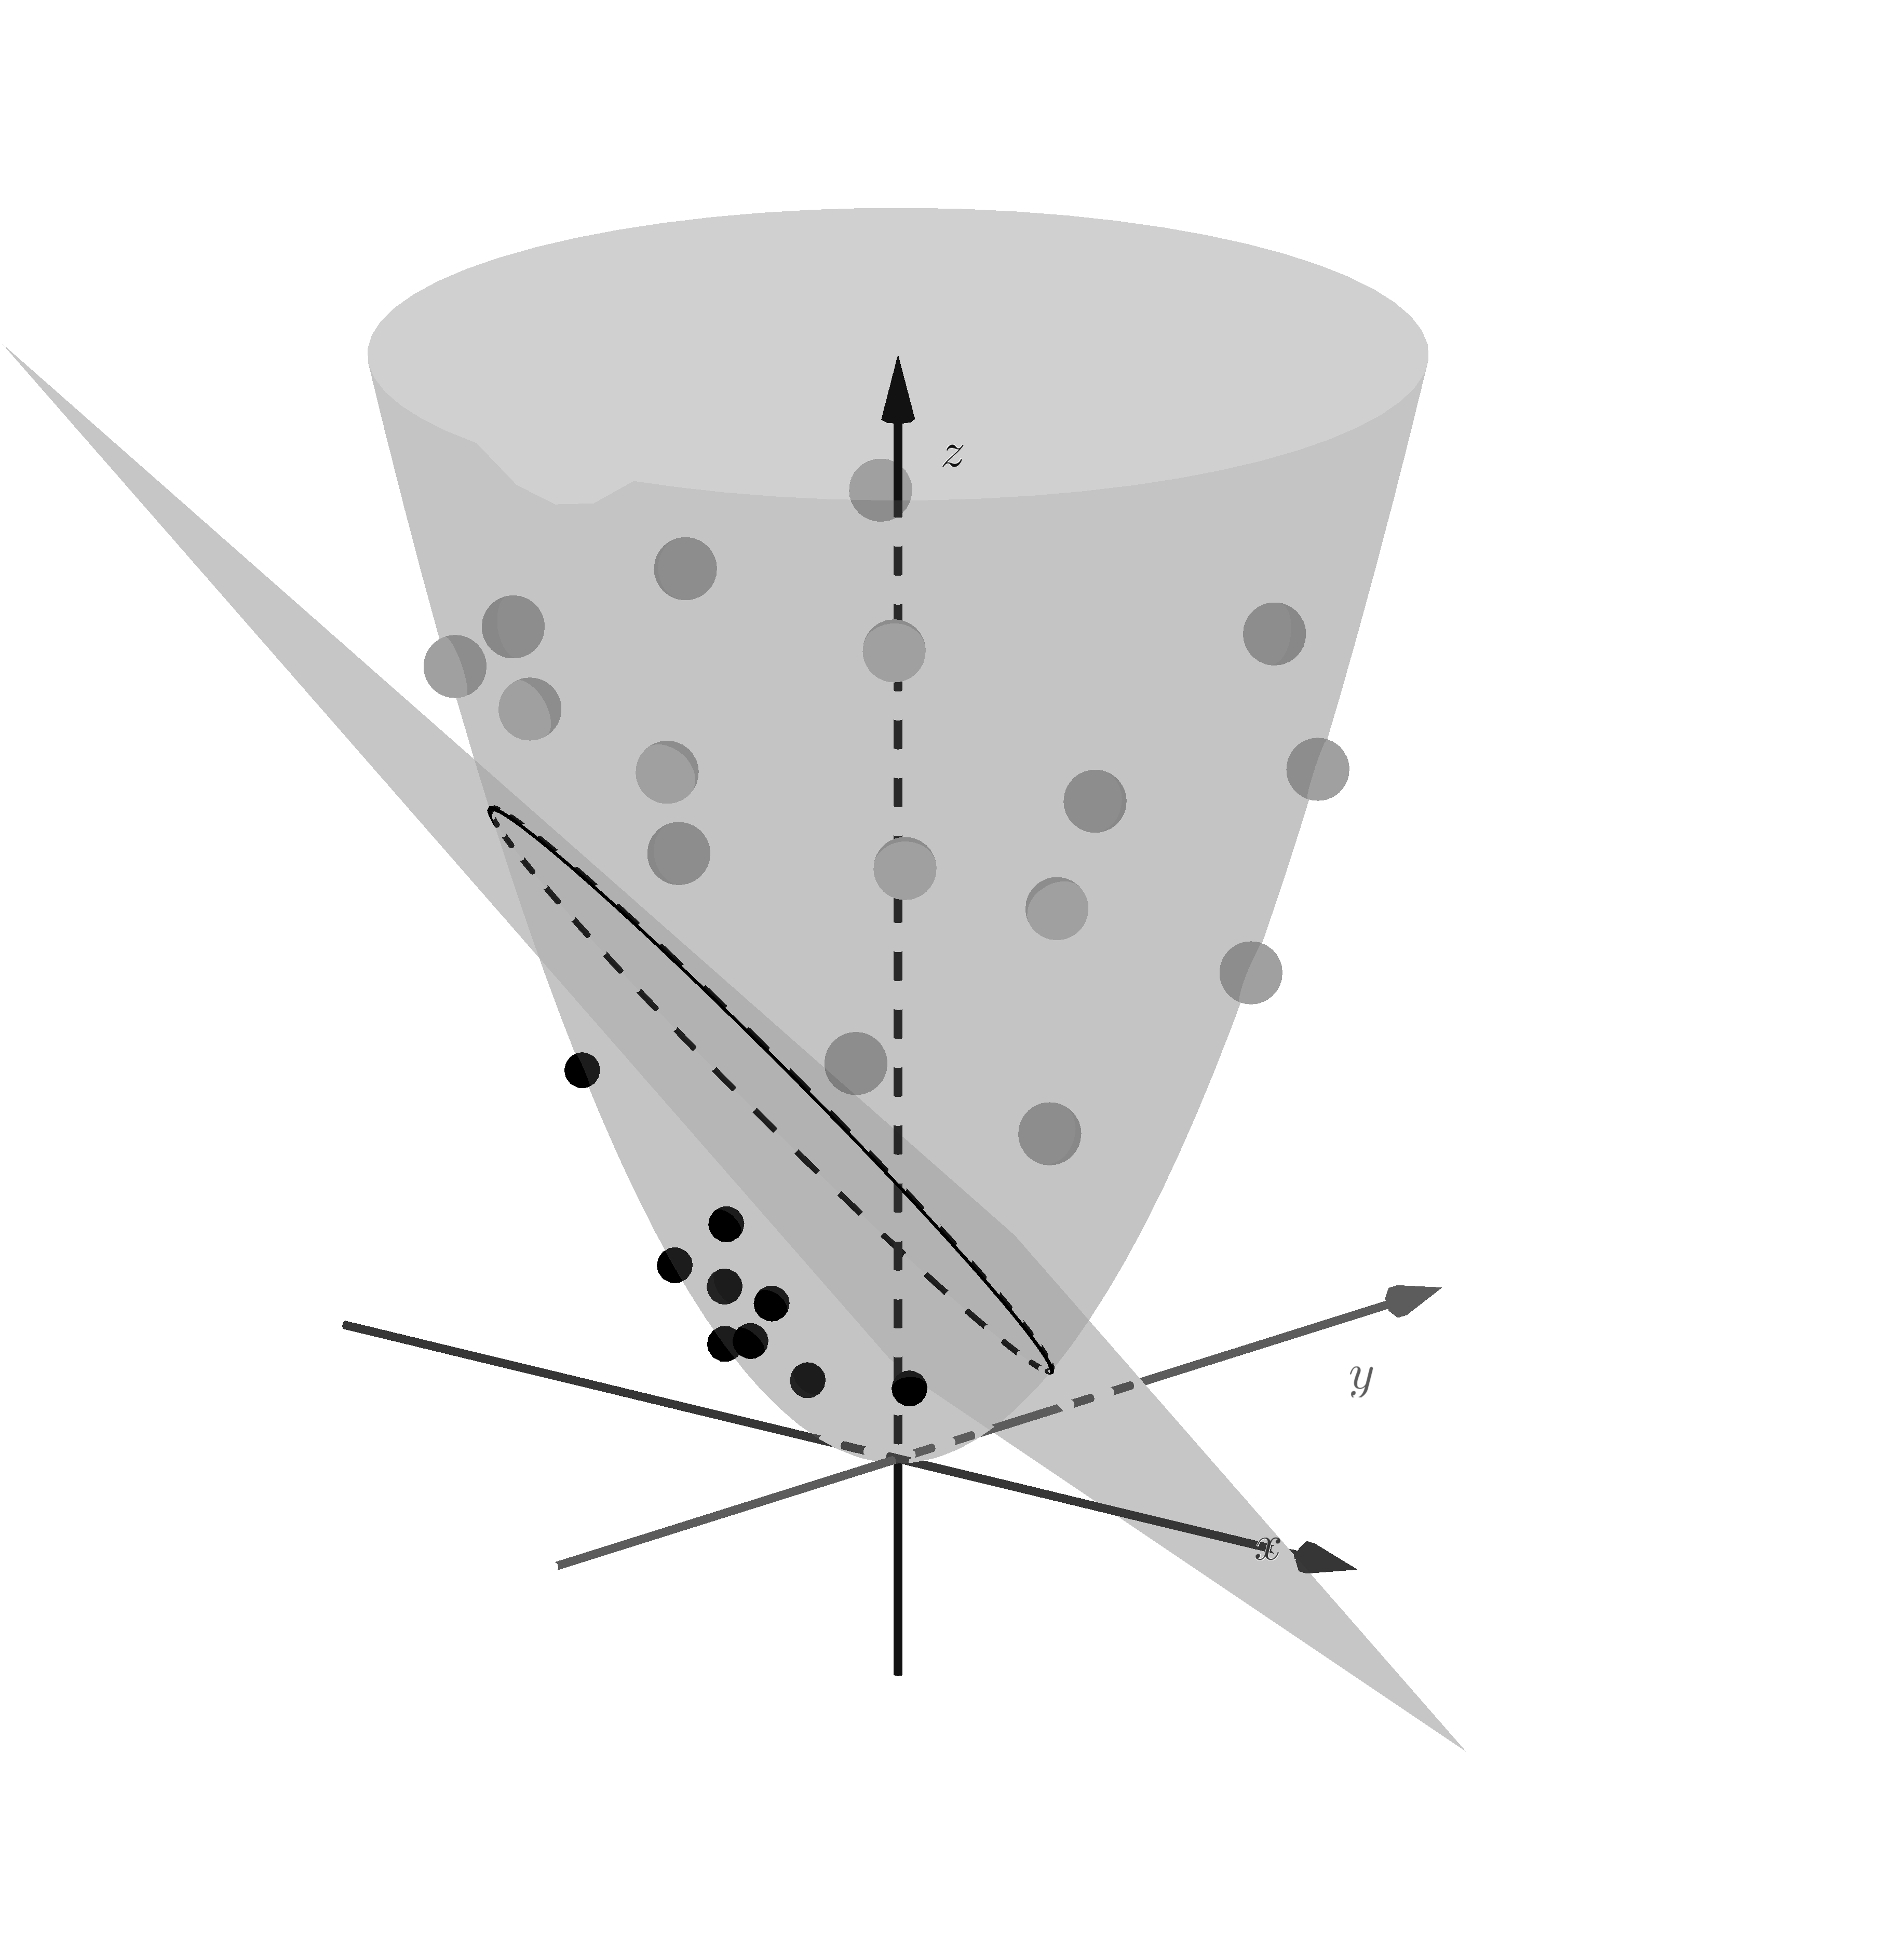
\includegraphics[width=\linewidth]{Chapters/09_SupportVectorMachines/21_kernelsvm/52_gray.png} %%%%
    \caption{}
    % \label{fig:subim2}
    \end{subfigure}
    \begin{subfigure}{0.325\textwidth}
    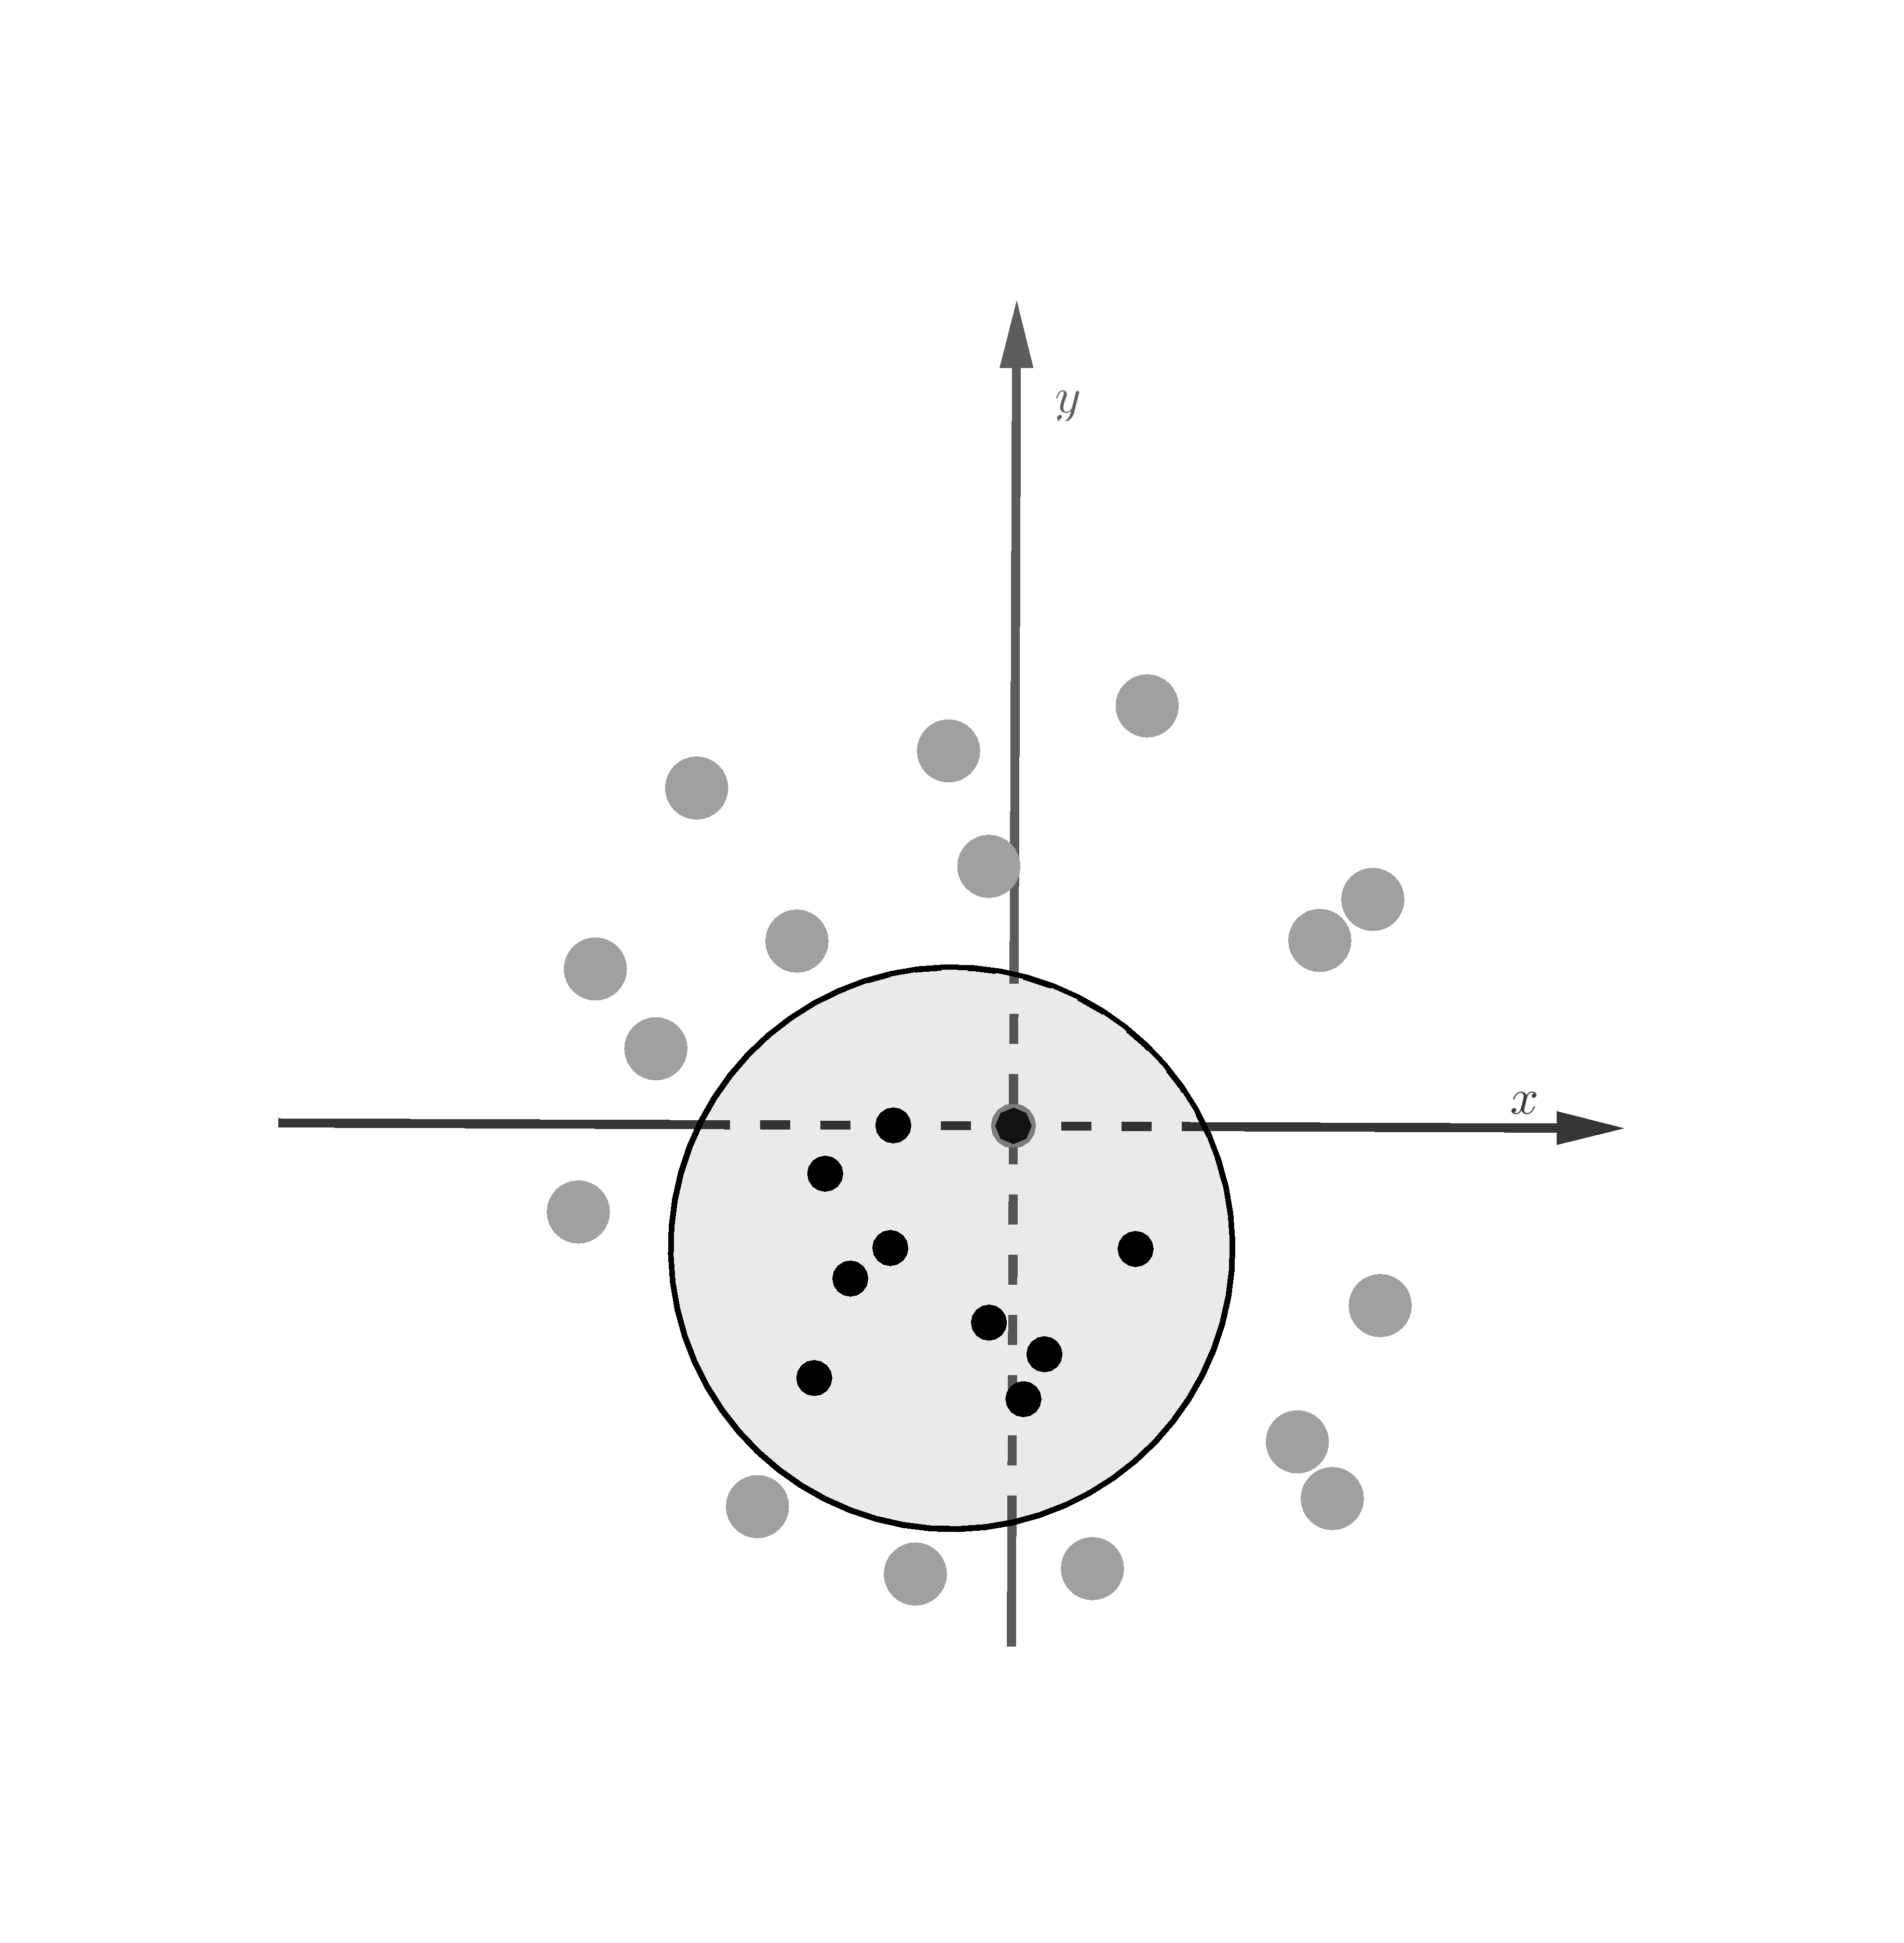
\includegraphics[width=\linewidth]{Chapters/09_SupportVectorMachines/21_kernelsvm/62_gray.png} %%%%
    \caption{}
    % \label{fig:subim2}
    \end{subfigure}

    \caption{
    Ví dụ về SVM hạt nhân. (a) Dữ liệu hai lớp không tách biệt tuyến tính trong không gian hai chiều. (b) Nếu xét thêm chiều thứ ba là một hàm số
    của hai chiều còn lại $z = x^2 + y^2$, các điểm dữ liệu sẽ được phân bố trên
    một mặt parabolic và hai lớp đã trở nên tách biệt tuyến tính. Mặt
    phẳng cắt prabolic chính là mặt phân chia, có thể tìm được bởi một 
    SVM lề cứng hoặc mềm. (c) Giao tuyến của mặt phẳng tìm được và mặt
    parabolic là một đường ellipse. Hình chiếu của đường ellipse này xuống không gian ban đầu chính là đường phân chia hai lớp dữ liệu.}
    \label{fig:21_1}
\end{figure}
% ******************************************************************************
Xét ví dụ trên Hình~\ref{fig:21_1} với việc biến dữ liệu không tách biệt tuyến tính trong không gian hai chiều thành tách biệt tuyến tính trong
không gian ba chiều. Để quan sát ví dụ này
một cách sinh động hơn, bạn có thể xem clip đi kèm trên blog \textit{Machine
Learning cơ bản} tại \url{https://goo.gl/3wMHyZ}.
 
% <div style="text-align:center;"> 
% <iframe width="600" height = "400" src="https://www.youtube.com/embed/04eOsL5vrWc" frameborder="0" allowfullscreen></iframe> 
% <div class="thecap">Một ví dụ về phương pháp kernel.</div> 
% </div> 
 
Nhìn từ góc độ toán học, SVM hạt nhân là phương pháp đi tìm một hàm số
$\Phi(\mathbf{x})$ biến đổi dữ liệu $\mathbf{x}$ từ không gian đặc trưng ban đầu
thành dữ liệu trong một không gian mới. Trong không gian mới, ta mong muốn dữ
liệu giữa hai lớp là (gần) tách biệt tuyến tính. Khi
đó, ta có thể dùng các bộ phân loại tuyến tính thông thường như hồi quy logistic/softmax hoặc SVM lề cứng/mềm. 

\index{hàm hạt nhân -- kernel function}

Các hàm $\Phi(\bx)$ thường tạo ra dữ liệu mới có số chiều lớn, thậm chí có thể vô hạn chiều. Nếu tính toán các hàm này trực tiếp,
chắc chắn chúng ta sẽ gặp các vấn đề về bộ nhớ và hiệu năng tính toán. Có một
cách tiếp cận khác là sử dụng các \textit{hàm số hạt nhân} (kernel function) mô tả quan hệ giữa hai
vector trong không gian mới thay vì tính toán trực tiếp biến
đổi của từng vector. Kỹ thuật này được xây dựng dựa
trên việc giải bài toán đối ngẫu trong SVM lề cứng/mềm.
 

Nếu phải so sánh, ta thấy rằng hàm hạt nhân có chức năng
tương tự như hàm kích hoạt trong mạng neuron vì chúng đều tạo ra các quan hệ phi tuyến.
% Trong Mục~\ref{sec:21_csth}, chúng ta cùng tìm hiểu cơ sở toán học của Kernel
% SVM, Mục~\ref{sec:21_kernelfns} sẽ giới thiệu một số hàm \textit{kernel}
% thường được sử dụng.
\newpage 
 
\section{Cơ sở toán học }
\label{sec:21_csth}
Cùng nhắc lại bài toán đối ngẫu trong SVM lề mềm cho dữ liệu gần tách biệt tuyến tính:
\begin{eqnarray} 
 \label{eqn:21_1}
\begin{aligned}
    \blambda &= \arg \max_{\blambda} \sum_{n=1}^N \lambda_n - \frac{1}{2} \sum_{n=1}^N\sum_{m=1}^N \lambda_n \lambda_m y_n y_m \mathbf{x}_n^T \mathbf{x}_m \\\      \text{thoả mãn:}~ & \sum_{n=1}^N \lambda_ny_n = 0\\\ 
     & 0 \leq \lambda_n \leq C, ~\forall n= 1, 2, \dots, N.
\end{aligned}
 \end{eqnarray} 
Trong đó, $N$ là số cặp điểm dữ liệu huấn luyện; $\mathbf{x}_n$ và $y_n = \pm 1$ lần lượt là là
vector đặc trưng và nhãn của dữ liệu thứ $n$; $\lambda_n$ là nhân tử Lagrange ứng
với điểm dữ liệu thứ $n$; và $C$ là một hằng số dương giúp cân đối độ lớn giữa độ rộng lề và sự hy sinh của các điểm nằm trong vùng không an toàn. Khi $C = \infty$ hoặc rất lớn, SVM lề mềm trở thành SVM lề cứng.

% \begin{itemize}
%     \item $N$: số cặp điểm dữ liệu trong tập huấn luyện.  
 
%     \item $\mathbf{x}_n$: vector đặc trưng của dữ liệu thứ $n$ trong tập
%     training.
 
%     \item $y_n$: \textit{nhãn} của điểm dữ liệu thứ $n$, bằng 1 hoặc -1. 
 
%     \item $\lambda_n$: nhân tử Lagrange ứng với điểm dữ liệu thứ $n$. 
 
%     \item $C$: một hằng số dương giúp cân đối độ lớn của \textit{margin} và
%     \textit{sự hy sinh} của các điểm nằm trong vùng \textit{không an toàn}. Khi $C = \infty$ hoặc rất lớn, soft-margin SVM trở thành hard-margin SVM.  
% \end{itemize}
 
Sau khi tìm được $\lambda$ cho bài toán \eqref{eqn:21_1}, nhãn của một điểm dữ liệu mới sẽ được xác định bởi 
\begin{equation} 
    \label{eqn:21_2}
    \text{class}(\bx) = \sgn \left\{\sum_{m \in \mathcal{S}} \lambda_m y_m
    \mathbf{x}_m^T \mathbf{x} + \frac{1}{N_{\mathcal{M}}} \sum_{n \in
    \mathcal{M}} \left(y_n - \sum_{m \in \mathcal{S}} \lambda_m y_m
    \mathbf{x}_m^T\mathbf{x}_n\right)\right\}
\end{equation} 
trong đó, $\mathcal{M} = \{n: 0 < \lambda_n < C\}$ là tập hợp những điểm nằm
trên hai đường thẳng hỗ trợ; $\mathcal{S} = \{n: 0 < \lambda_n\}$ là tập hợp
các vector nằm trên hai đường hỗ trợ hoặc nằm giữa chúng; $N_{\mathcal{M}}$ là số phần tử của
$\mathcal{M}$.

Rất hiếm khi dữ liệu thực tế {gần tách biệt tuyến tính}, vì
vậy nghiệm của bài toán \eqref{eqn:21_1} có thể không thực sự tạo ra một bộ phân
loại tốt. Giả sử rằng ta có thể tìm được hàm số $\Phi()$ sao cho các điểm dữ liệu $\Phi(\bx)$ trong không gian mới (gần) tách biệt tuyến tính. 
 
Trong không gian mới, bài toán \eqref{eqn:21_1} trở thành:  
 \begin{eqnarray} 
 \label{eqn:21_3}
 \begin{aligned}
     \blambda &= \arg \max_{\blambda} \sum_{n=1}^N \lambda_n - \frac{1}{2} \sum_{n=1}^N\sum_{m=1}^N \lambda_n \lambda_m y_n y_m \Phi(\mathbf{x}_n)^T \Phi(\mathbf{x}_m)\\\ 
     \text{thoả mãn:}~ & \sum_{n=1}^N \lambda_ny_n = 0 \\\ 
     & 0 \leq \lambda_n \leq C, ~\forall n= 1, 2, \dots, N  
 \end{aligned}
 \end{eqnarray} 
Nhãn của một điểm dữ liệu mới được xác định bởi dấu của biểu thức:
\begin{equation} 
    \label{eqn:21_4}
    \mathbf{w}^T\Phi(\mathbf{x}) + b = \sum_{m \in \mathcal{S}} \lambda_m y_m \Phi(\mathbf{x}_m)^T \Phi(\mathbf{x}) + \frac{1}{N_{\mathcal{M}}} \sum_{n \in \mathcal{M}} \left(y_n - \sum_{m \in \mathcal{S}} \lambda_m y_m \Phi(\mathbf{x}_m)^T\Phi(\mathbf{x}_n)\right)
\end{equation} 
 
Như đã đề cập, việc tính toán trực tiếp $\Phi(\mathbf{x})$ cho mỗi điểm dữ
liệu có thể sẽ tốn rất nhiều bộ nhớ và thời gian vì số chiều của $\Phi(\mathbf{x})$ thường rất lớn, có thể là vô hạn. Thêm nữa, để tìm {nhãn} của một điểm dữ liệu mới $\mathbf{x}$, ta cần tính $\Phi(\mathbf{x})$ rồi lấy tích vô hướng với các $\Phi(\mathbf{x}_m), m \in \mathcal{S}$. Việc tính toán này có thể được hạn chế bằng quan sát dưới đây.  

% \index{Kernel}
\index{thủ thuật hạt nhân -- kernel trick} 
Trong bài toán \eqref{eqn:21_3} và biểu thức \eqref{eqn:21_4}, ta không
cần tính trực tiếp $\Phi(\mathbf{x})$ cho mọi điểm dữ liệu. Thay vào đó, ta chỉ cần
tính $\Phi(\mathbf{x})^T\Phi(\mathbf{z})$ với hai điểm dữ liệu
$\mathbf{x}, \mathbf{z}$. Vì vậy, ta không cần xác định hàm
$\Phi(.)$ mà chỉ cần tính giá trị $k(\bx, \bz) = \Phi(\bx)^T\Phi(\bz)$. Kỹ thuật tính tích vô hướng của hai điểm trong không gian mới thay vì tọa độ của từng điểm có tên gọi chung là \textit{thủ thuật hạt nhân} (kernel trick).
 
Bằng cách định nghĩa hàm hạt nhân $k(\mathbf{x}, \mathbf{z}) =
\Phi(\mathbf{x})^T\Phi(\mathbf{z}) $, ta có thể viết lại bài toán
\eqref{eqn:21_3} và biểu thức \eqref{eqn:21_4} như sau:
\begin{eqnarray} 
\label{eqn:21_5}
\begin{aligned}
    \blambda &= \arg \max_{\blambda} \sum_{n=1}^N \lambda_n - \frac{1}{2} \sum_{n=1}^N\sum_{m=1}^N \lambda_n \lambda_m y_n y_m k(\mathbf{x}_n,\mathbf{x}_m)\\\ 
    \text{thoả mãn:}~ &\sum_{n=1}^N \lambda_ny_n = 0\\\ 
    & 0 \leq \lambda_n \leq C, ~\forall n= 1, 2, \dots, N 
\end{aligned}
\end{eqnarray} 
và
\begin{equation} 
    \label{eqn:21_6}
    \sum_{m \in \mathcal{S}} \lambda_m y_m k(\mathbf{x}_m, \mathbf{x}) + \frac{1}{N_{\mathcal{M}}} \sum_{n \in \mathcal{M}} \left(y_n - \sum_{m \in \mathcal{S}} \lambda_m y_m k(\mathbf{x}_m, \mathbf{x}_n)\right)
\end{equation} 
 
\textit{Ví dụ}: Xét phép biến đổi một điểm trong không gian hai chiều
$\mathbf{x} = [x_1, x_2]^T$ thành một điểm trong không gian năm chiều
$\Phi(\mathbf{x}) = [1, \sqrt{2} x_1, \sqrt{2} x_2, x_1^2, \sqrt{2} x_1x_2,
x_2^2]^T$. Ta có:
\begin{eqnarray*} 
\Phi(\mathbf{x})^T\Phi(\mathbf{z}) &=& [1, \sqrt{2} x_1, \sqrt{2} x_2, x_1^2, \sqrt{2} x_1x_2, x_2^2] [1, \sqrt{2} z_1, \sqrt{2} z_2, z_1^2, \sqrt{2} z_1z_2, z_2^2]^T \\\ 
&=& 1 + 2x_1z_1 + 2x_2z_2 + x_1^2x_2^2 + 2x_1z_1x_2z_2 + x_2^2z_2^2 \\\ 
&=& (1 + x_1z_1 + x_2z_2)^2 = (1 + \mathbf{x}^T\mathbf{z})^2 = k(\mathbf{x}, \mathbf{z}) 
\end{eqnarray*} 
Trong ví dụ này, việc tính toán hàm hạt nhân $k(\bx, \bz) = (1 +
\bx^T\bz)^2$ cho hai điểm dữ
liệu đơn giản hơn việc tính từng $\Phi(.)$ rồi nhân chúng với nhau. Hơn nữa, giá
trị thu được là một số vô hướng thay vì hai vector năm chiều
$\Phi(\bx), \Phi(\bz)$. 
 
Hàm hạt nhân cần có những tính chất gì, và những hàm nào được sử dụng phổ biến?  
 
% \newpage 
\section{Hàm số hạt nhân}
\label{sec:21_kernelfns}
\index{hàm hạt nhân -- kernel function}
 
\subsection{Tính chất của các hàm hạt nhân }
Không phải hàm $k()$ nào cũng có thể được sử dụng. Các hàm hạt nhân cần có các tính chất: 
\index{die@điều kiện Mercer}
\begin{itemize}
    \item Đối xứng: $k(\mathbf{x}, \mathbf{z}) = k(\mathbf{z}, \mathbf{x})$, vì
    tích vô hướng của hai vector có tính đối xứng. 
     
    \item {Về lý thuyết}, hàm kernel cần thỏa mãn điều kiện
    Mercer\footnote{Xem \textit{Kernel method -- Wikipedia}
    (\url{https://goo.gl/YXct7F})}:
    \begin{equation} 
    \label{eqn:21_7}
    \sum_{n=1}^N \sum_{m=1}^N k(\mathbf{x}_m, \mathbf{x}_n) c_nc_m \geq 0, ~~ \forall c_i \in \mathbb{R}, i = 1, 2, \dots, N 
    \end{equation} 
    với mọi tập hữu hạn các vector $\bx_1, \dots, \bx_N$. 
    Tính chất này giúp đảm bảo hàm mục tiêu trong bài toán đối ngẫu
    \eqref{eqn:21_5} là {lồi}. Thật vậy, nếu một hàm kernel thỏa mãn điều
    kiện \eqref{eqn:21_7}, xét $c_n = y_n \lambda_n$, ta sẽ có:  
    \begin{equation} 
    \label{eqn:21_8}
    \blambda^T \mathbf{K} \blambda = \sum_{n=1}^N \sum_{m=1}^N k(\mathbf{x}_m, \mathbf{x}_n) y_ny_m \lambda_n \lambda_m \geq 0, ~\forall \lambda_n 
    \end{equation} 
    với $\mathbf{K}$ là một ma trận đối xứng và $ k_{nm} = y_ny_m k(\mathbf{x}_n, \mathbf{x}_m) $.
    Từ \eqref{eqn:21_8} ta suy ra $\mathbf{K}$ là một ma trận nửa xác định dương. Vì vậy, bài toán tối ưu \eqref{eqn:21_5} có ràng buộc là lồi và hàm mục tiêu là một hàm lồi (một quy hoạch toàn phương). Điều kiện này giúp bài toán được giải một cách hiệu quả.  

    \item {Trong thực hành}, một vài hàm số $k()$ không thỏa mãn điều
    kiện Mercer vẫn cho kết quả chấp nhận được. Những hàm số này vẫn được
    gọi là hạt nhân. Trong chương này, chúng ta chỉ quan tâm tới các hàm
    hạt nhân thông dụng có sẵn trong các thư viện.
\end{itemize}
 
Việc giải quyết bài toán~\eqref{eqn:21_5} hoàn toàn tương tự như bài toán
đối ngẫu trong SVM lề mềm. Chúng ta sẽ không đi sâu vào việc tính nghiệm này. Thay
vào đó, chúng ta sẽ thảo luận các hàm hạt nhân thông dụng và hiệu năng của chúng trong các bài toán.
 
\subsection{Một số hàm hạt nhân thông dụng}
\index{hàm hạt nhân -- kernel function!tuyến tính -- linear}
\subsubsection{Tuyến tính}
Đây là trường hợp đơn giản với hàm hạt nhân chính là tích vô hướng của hai vector:  
$k(\mathbf{x}, \mathbf{z}) = \mathbf{x}^T\mathbf{z}$.
Như đã chứng minh trong Chương~\ref{cha:svm}, hàm số thỏa mãn điều kiện \eqref{eqn:21_7}. Khi sử dụng \pythoninline{sklearn.svm.SVC}, hàm này được chọn bằng cách gán 
\pythoninline{kernel = 'linear'}. 
 
 
\subsubsection{Đa thức}
\index{hàm hạt nhân -- kernel function!đa thức -- polynomial}
Hàm hạt nhân đa thức có dạng 
\begin{equation} 
k(\mathbf{x}, \mathbf{z}) = (r + \gamma \mathbf{x}^T\mathbf{z})^d 
\end{equation} 
Với $d$ là một số thực dương. Khi $d$ là một số tự nhiên, hạt nhân đa thức có thể mô tả hầu hết các đa thức có bậc không
vượt quá $d$.

Khi sử dụng thư viện \pythoninline{sklearn}, hạt nhân này được chọn bằng cách gán
\pythoninline{kernel = 'poly'}. Bạn đọc có thể tìm thấy tài liệu
chính thức trong scikit-learn tại \url{https://goo.gl/QvtFc9}. 
 
\subsubsection{Hàm cơ sở radial}
\index{hàm cơ sở radial -- radial basic function, RBF}
\index{hàm hạt nhân -- kernel function!RBF}
\textit{Hàm cơ sở radial} (radial basic function, RBF hay hạt nhân Gauss) là lựa chọn mặc định trong sklearn, được sử dụng nhiều nhất trong thực tế. Hàm số này được định nghĩa bởi
\begin{equation} 
k(\mathbf{x}, \mathbf{z}) = \exp(-\gamma \|\mathbf{x} - \mathbf{z}\|_2^2), ~~ \gamma > 0 
\end{equation}  
 
\subsubsection{Sigmoid }
\index{hàm hạt nhân -- kernel function!sigmoid}
Hàm dạng sigmoid cũng được sử dụng làm hạt nhân:
\begin{equation} 
k(\mathbf{x}, \mathbf{z}) = \text{tanh}(\gamma \mathbf{x}^T\mathbf{z} + r) 
\end{equation} 
Trong \pythoninline{sklearn}, hạt nhân này được lựa chọn bằng cách gán \pythoninline{kernel
= 'sigmoid'}.
 
 
\subsubsection{Bảng tóm tắt các hàm hạt nhân thông dụng }
 
Bảng~\ref{tab:21_2} tóm tắt các hàm hạt nhân thông dụng và cách sử dụng trong
\pythoninline{sklearn}.  
 
\begin{table}[h!]
\centering
\caption{Bảng các hàm hạt nhân thông dụng}
\label{tab:21_2}
\def\arraystretch{1.5}
\setlength\tabcolsep{5pt}
\begin{tabular}{|l|l|l|l|}
\hline
\textbf{Tên }& \textbf{Công thức} & \textbf{Thiết lập hệ số} \\ \hline
\pythoninline{'linear'}     & $\mathbf{x}^T\mathbf{z}$                            & không có hệ số                                             \\ \hline
\pythoninline{'poly'}  & $(r + \gamma \mathbf{x}^T\mathbf{z})^d $         &     $d$: \pythoninline{degree}, $\gamma$: \pythoninline{gamma}, $r$: \pythoninline{coef0} \\ \hline 
\pythoninline{'sigmoid'}    & $\text{tanh}(\gamma \mathbf{x}^T\mathbf{z} + r)$ &   $\gamma$: \pythoninline{gamma}, $r$: \pythoninline{coef0}                    \\ \hline 
\pythoninline{'rbf'}         & $\exp(-\gamma \&\mathbf{x} - \mathbf{z}\&_2^2)$           & $\gamma >0$: \pythoninline{gamma}     \\ \hline 
\end{tabular}
\end{table}

Nếu muốn sử dụng các thư viện cho C/C++, các bạn có thể tham khảo LIBSVM
(\url{https://goo.gl/Dt7o7r}) và {LIBLINEAR} (\url{https://goo.gl/ctD7a3}).
 
 
\subsubsection{Hàm tự định nghĩa }
 
Ngoài các hàm hạt nhân thông dụng như trên, chúng ta cũng có thể tự định nghĩa các
hàm hạt nhân theo hướng dẫn tại \url{https://goo.gl/A9ajzp}.

\section{Ví dụ minh họa}
 
 
\subsection{Bài toán XOR}
Chúng ta biết rằng bài toán XOR không
thể giải quyết nếu chỉ dùng một bộ phân loại tuyến tính. Trong mục này, chúng ta sẽ thử ba hàm hạt nhân khác nhau và sử dụng SVM. Kết quả được minh hoạ trong Hình \ref{fig:21_2}. Dưới đây là đoạn mã tìm các mô hình tương ứng:

\begin{lstlisting}[language=Python]
import numpy as np
import matplotlib.pyplot as plt
from sklearn import svm

# XOR dataset and targets
X = np.array([[0, 0], [1, 1], [1, 0], [0, 1]])
y = np.array([0, 0, 1, 1])
# fit the model
for kernel in ('sigmoid', 'poly', 'rbf'):
    clf = svm.SVC(kernel=kernel, gamma=4, coef0 = 0)
    clf.fit(X, y)
\end{lstlisting}
% 
 
% ******************************************************************************
\begin{figure}[t]
    \begin{subfigure}{0.325\textwidth}
    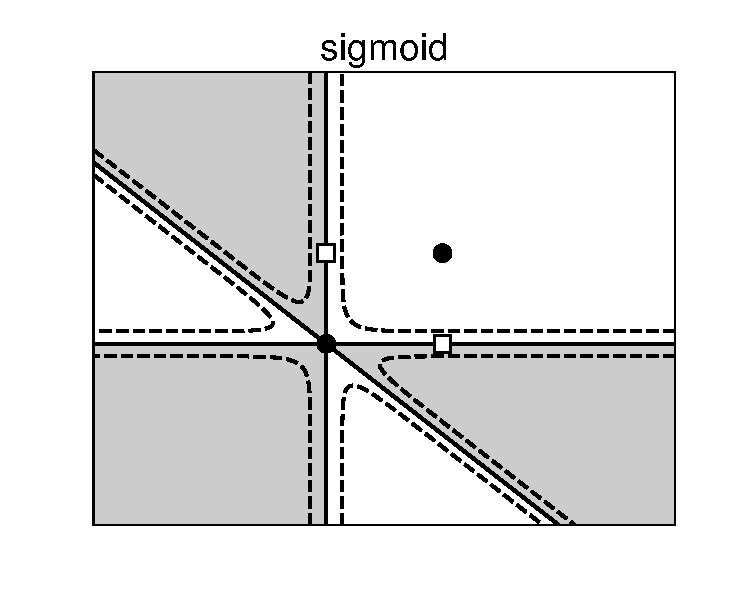
\includegraphics[width=\linewidth]{Chapters/09_SupportVectorMachines/21_kernelsvm/plt/sigmoid1.pdf}
    \caption{hạt nhân sigmoid}
    % \label{fig:subim1}
    \end{subfigure}
    \begin{subfigure}{0.325\textwidth}
    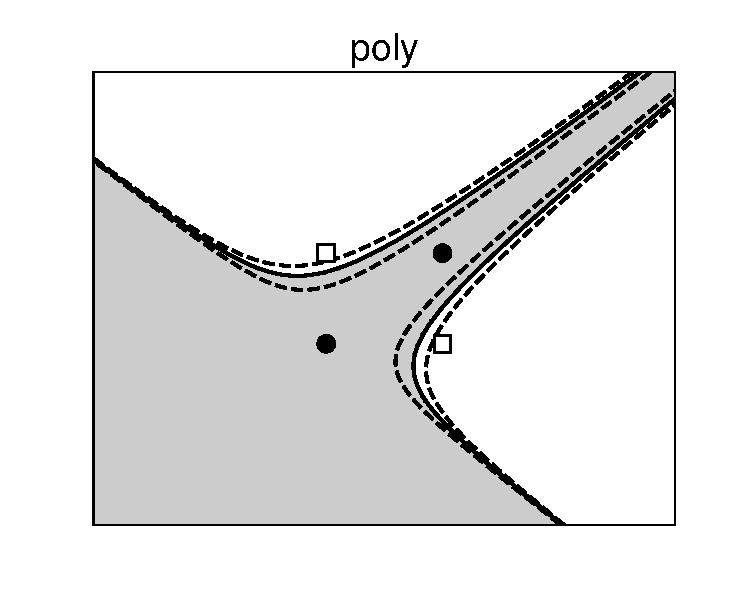
\includegraphics[width=\linewidth]{Chapters/09_SupportVectorMachines/21_kernelsvm/plt/poly1.pdf}
    \caption{hạt nhân đa thức}
    % \label{fig:subim2}
    \end{subfigure}
    \begin{subfigure}{0.325\textwidth}
    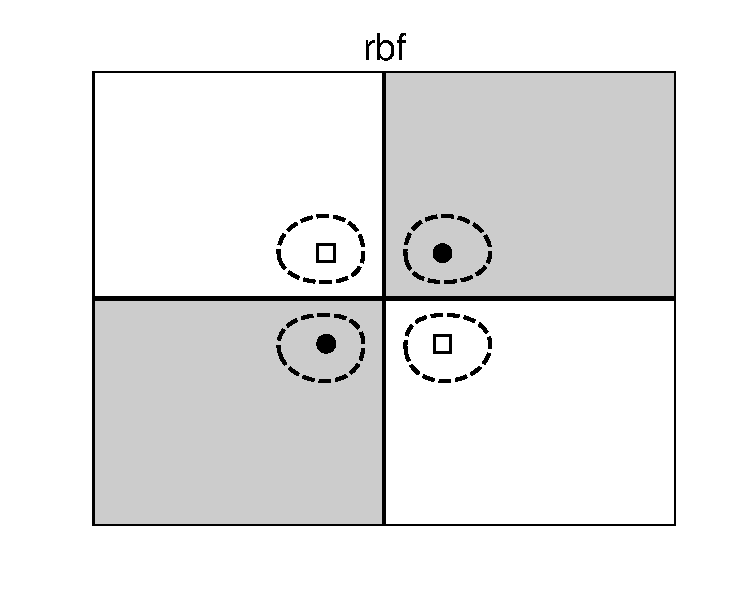
\includegraphics[width=\linewidth]{Chapters/09_SupportVectorMachines/21_kernelsvm/plt/rbf1.pdf}
    \caption{hạt nhân rbf}
    % \label{fig:subim2}
    \end{subfigure}

    \caption{
    Sử dụng SVM hạt nhân để giải quyết bài toán XOR: (a) hạt nhân sigmoid, (b)
 hạt nhân đa thức, (c) hạt nhân RBF. Các đường nét liền là các đường phân loại,
    ứng với giá trị của biểu thức \eqref{eqn:21_6} bằng 0. Các đường nét đứt là
    các đường đồng mức ứng với giá trị của biểu thức \eqref{eqn:21_6} bằng $\pm
    0.5$. Các vùng có nền màu xám tương ứng với lớp các điểm đen hình tròn, các
    vùng có nền trắng tương ứng với lớp các điểm trắng hình vuông. Trong ba
    hạt nhân, RBF cho kết quả đối xứng, hợp lý
    với dữ liệu bài toán. }
    \label{fig:21_2}
\end{figure}
% ******************************************************************************
 
Nhận xét với mỗi hàm hạt nhân: 
\begin{itemize}
    \item \pythoninline{sigmoid}: Nghiệm tìm được không thật tốt vì có ba trong
    bốn điểm nằm chính xác trên các đường phân chia. 

    \item \pythoninline{poly}: Nghiệm này tốt hơn nghiệm của
    \pythoninline{sigmoid} nhưng kết quả có phần quá khớp. 
     
    \item \pythoninline{rbf}: Đường phân
    chia tìm được khá hợp lý khi tạo ra các vùng đối xứng phù hợp với dữ liệu. Trên thực tế, các \pythoninline{rbf} kernel được sử dụng nhiều nhất và cũng là lựa chọn mặc định trong \pythoninline{sklearn.svm.SVC}. 
\end{itemize}
 
 
\subsection{Dữ liệu gần tách biệt tuyến tính}
 
Xét một ví dụ khác với dữ liệu giữa hai lớp gần tách biệt tuyến tính như trong Hình~\ref{fig:21_3}. Trong ví dụ này, dường như quá khớp đã xảy ra với \pythoninline{kernel = 'rbf'}. Hạt nhân \pythoninline{sigmoid} cho kết quả không thực sự tốt và ít được sử dụng.  
 
 
% \subsection{Bài toán phân biệt giới tính}
% Bài toán này đã được đề cập ở Bài 12 với dữ liệu đầu vào là các ảnh khuôn mặt. Vì tôi không được phép phân phối cơ sở dữ liệu gốc này, tôi sẽ chia sẻ cho các bạn về dữ liệu đã qua xử lý, được lưu trong file \pythoninline{myARgender.mat}, có thể được \href{https://github.com/tiepvupsu/tiepvupsu.github.io/blob/master/assets/21_kernelsvm/plt/myARgender.mat}{download tại đây}. Dưới đây là ví dụ về cách sử dụng thư viện \pythoninline{sklearn.svm.SVC} để giải quyết bài toán: 
% ******************************************************************************
\begin{figure}[t]
    \begin{subfigure}{0.325\textwidth}
    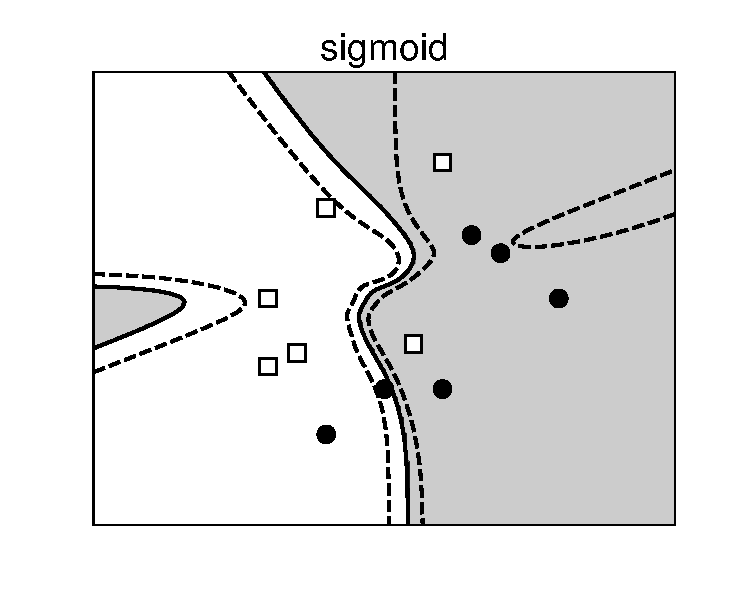
\includegraphics[width=\linewidth]{Chapters/09_SupportVectorMachines/21_kernelsvm/plt/sigmoid3.pdf}
    \caption{sigmoid kernel.}
    % \label{fig:subim1}
    \end{subfigure}
    \begin{subfigure}{0.325\textwidth}
    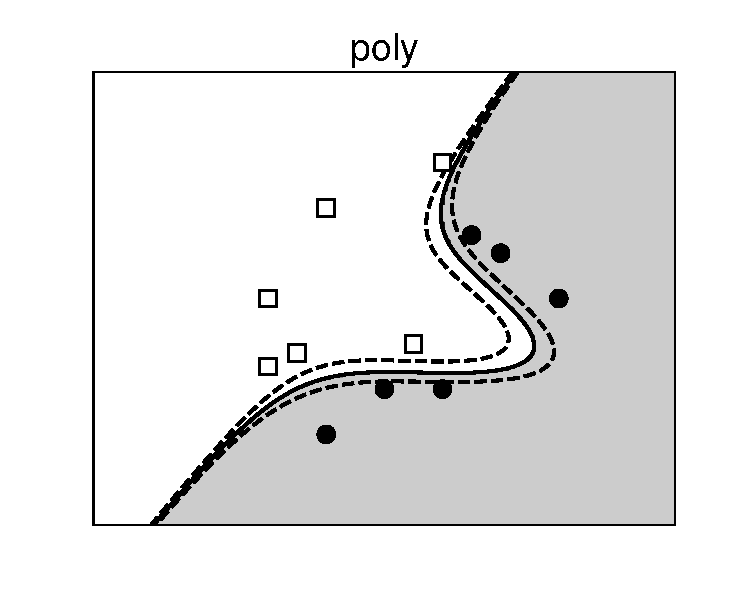
\includegraphics[width=\linewidth]{Chapters/09_SupportVectorMachines/21_kernelsvm/plt/poly3.pdf}
    \caption{poly kernel.}
    % \label{fig:subim2}
    \end{subfigure}
    \begin{subfigure}{0.325\textwidth}
    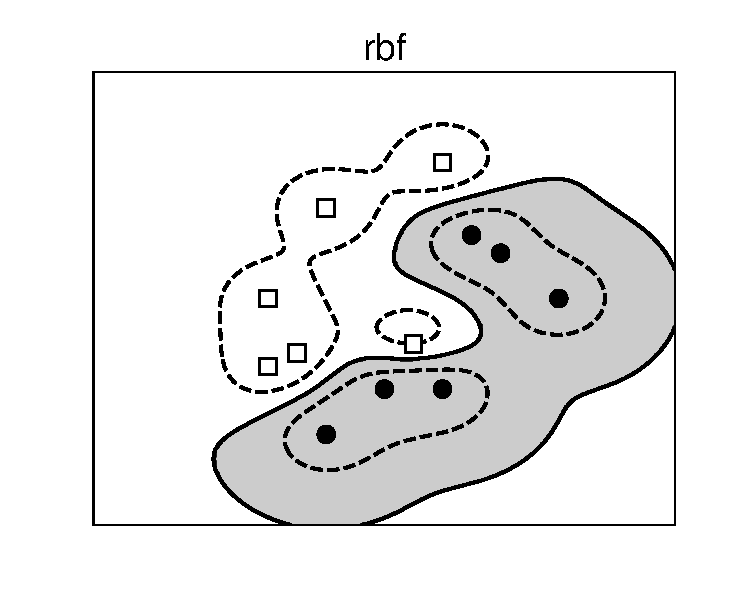
\includegraphics[width=\linewidth]{Chapters/09_SupportVectorMachines/21_kernelsvm/plt/rbf3.pdf}
    \caption{rbf kernel.}
    % \label{fig:subim2}
    \end{subfigure}

    \caption{
    Sử dụng SVM hạt nhân giải quyết bài toán với dữ liệu {gần tách biệt
    tuyến tính}: (a) hạt nhân sigmoid, (b) hạt nhân đa thức, (c) hạt nhân RBF. Hạt nhân đa thức cho kết quả hợp lý nhất. }
    \label{fig:21_3}
\end{figure}
% ******************************************************************************
% \newpage
 
% \begin{lstlisting}[language=Python]
% import scipy.io as sio 
% from sklearn.svm import SVC 
 
% A = sio.loadmat('myARgender.mat') 
% X_train = A['Y_train'].T  
% X_test = A['Y_test'].T  
% N = 700 
% y_train = A['label_train'].reshape(N) 
% y_test = A['label_test'].reshape(N) 
 
% clf = SVC(kernel='poly', degree = 3, gamma=1, C = 100) 
% clf.fit(X_train, y_train) 
% y_pred = clf.predict(X_test) 
% print("Accuracy: %.2f %%" %(100*accuracy_score(y_test, y_pred))) 
% \end{lstlisting}
 
% \begin{lstlisting}[language=Python]
% Accuracy: 92.86 % 
% \end{lstlisting}
 
% Kết quả không tệ! Các bạn thử thay các \pythoninline{kernel} và thiết lập các tham số khác xem kết quả thay đổi như thế nào. Vì dữ liệu giữa hai classes là \textit{gần phân biệt tuyến tính} nên không có sự khác nhau nhiều giữa các kernel. 
 
\subsection{Máy vector hỗ trợ hạt nhân cho MNIST}
Tiếp theo, chúng ta áp dụng SVM với hạt nhân RBF vào bài toán phân loại bốn chữ số \pythoninline{0, 1, 2, 3} của cơ sở dữ liệu chữ số viết tay MNIST.
Trước hết, chúng ta cần lấy dữ liệu rồi chuẩn hóa về đoạn $[0, 1]$ bằng cách chia toàn bộ các thành phần cho 255 (giá trị cao
nhất của mỗi điểm ảnh): 
\begin{lstlisting}[language=Python]
from __future__ import print_function 
import numpy as np 
from sklearn import svm
from sklearn.datasets import fetch_mldata
data_dir = '../../data' # path to your data folder 
mnist = fetch_mldata('MNIST original', data_home=data_dir)

X_all = mnist.data/255. # data normalization 
y_all = mnist.target 
digits = [0, 1, 2, 3]
ids = []
for d in digits:
    ids.append(np.where(y_all == d)[0])

selected_ids = np.concatenate(ids, axis = 0)
X = X_all[selected_ids]
y = y_all[selected_ids]
print('Number of samples = ', X.shape[0])
\end{lstlisting}
\kq 
\begin{lstlisting}[language=Python]
Number of samples =  28911
\end{lstlisting}
Như vậy, tổng cộng có khoảng 29000 điểm dữ liệu. Chúng ta lấy ra 24000
điểm làm tập kiểm tra, còn lại là dữ liệu huấn luyện. Sử dụng bộ phân loại SVM hạt nhân:
\begin{lstlisting}[language=Python]
from sklearn.model_selection import train_test_split
from sklearn.metrics import accuracy_score
X_train, X_test, y_train, y_test = train_test_split(X, y, test_size= 24000)

model = svm.SVC(kernel='rbf', gamma=.1, coef0 = 0)
model.fit(X_train, y_train)
y_pred = model.predict(X_test) 
print("Accuracy: %.2f %%" %(100*accuracy_score(y_test, y_pred))) 
\end{lstlisting}
\kq 
\begin{lstlisting}[language=Python]
Accuracy: 94.22 %
\end{lstlisting}
Kết quả thu được là khoảng 94\%. Nếu chọn nhiều điểm dữ liệu huấn luyện hơn và
thay đổi các tham số \pythoninline{gamma, coef0}, bạn đọc có thể sẽ thu được
kết quả tốt hơn. Đây là một bài toán phân loại đa lớp, và
kỹ thuật giải quyết của thư viện này là \textit{one-vs-rest}. Như đã đề cập trong
Chương~\ref{cha:logisticregression}, \textit{one-vs-rest} có nhiều hạn chế vì
phải huấn luyện nhiều bộ phân loại. Hơn nữa, với SVM hạt nhân, việc tính toán các
hàm hạt nhân cũng trở nên phức tạp khi lượng dữ liệu và số chiều dữ liệu tăng lên.


\section{Tóm tắt }

\begin{itemize}
    \item Trong bài toán phân loại nhị phân, nếu dữ liệu hai lớp {không tách biệt tuyến tính}, chúng ta có thể tìm cách biến đổi dữ liệu sao cho chúng (gần) tách biệt tuyến tính trong không gian mới. 
     
    \item Việc tính toán trực tiếp hàm $\Phi()$ đôi khi phức tạp và tốn nhiều bộ nhớ. Thay vào đó, ta có thể sử dụng thủ thuật hạt nhân. Trong cách tiếp cận này, ta chỉ cần tính tích vô hướng của hai vector bất kỳ trong không gian mới: $k(\mathbf{x}, \mathbf{z}) = \Phi(\mathbf{x})^T\Phi(\mathbf{z})$. 
    Thông thường, các hàm $k(., .)$ thỏa mãn điều kiện Mercer, và được
    gọi là hàm hạt nhân. Cách giải bài toán SVM với hàm hạt nhân hoàn toàn giống cách giải bài toán tối ưu trong SVM lề mềm. 
     
    \item Có bốn hàm hạt nhân thông dụng: \pythoninline{linear},
    \pythoninline{poly}, \pythoninline{rbf}, \pythoninline{sigmoid}. Trong đó, \pythoninline{rbf} được sử dụng nhiều nhất và là lựa chọn mặc định trong các thư viện SVM.
     
    \item Mã nguồn cho chương này có thể được tìm thấy tại \url{https://goo.gl/6sbds5}.
     
\end{itemize}
 
 
% \section{Tài liệu tham khảo }
% [1] Bishop, Christopher M. ``\href{https://www.amazon.com/Pattern-Recognition-Learning-Information-Statistics/dp/0387310738}{Pattern recognition and Machine Learning.}'', Springer  (2006).
 
% [2] Duda, Richard O., Peter E. Hart, and David G. Stork. Pattern classification. John Wiley \& Sons, 2012. 
 
% [3] \href{http://scikit-learn.org/stable/modules/generated/sklearn.svm.SVC.html}{\pythoninline{sklearn.svm.SVC}} 
 
% [4] \href{https://www.csie.ntu.edu.tw/~cjlin/libsvm/}{LIBSVM  --  A Library for Support Vector Machines} 
 
% [5] Bennett, K. P. (1992). "\href{http://citeseerx.ist.psu.edu/viewdoc/download?doi=10.1.1.23.3307&rep=rep1&type=pdf}{Robust linear programming discrimination of two linearly separable sets}". \textit{Optimization Methods and Software} 1, 23–34. 
 
% % [6] Sch¨olkopf, B., A. Smola, R. C.Williamson, and P. L. Bartlett (2000). "\href{http://citeseerx.ist.psu.edu/viewdoc/download?doi=10.1.1.94.2928&rep=rep1&type=pdf}{New support vector algorithms}". \textit{Neural Computation 12_(5), 1207–1245 

% [6] Schölkopf, Bernhard, et al. ``\href{https://www.google.com/url?sa=t&rct=j&q=&esrc=s&source=web&cd=1&cad=rja&uact=8&ved=0ahUKEwiEkdf_yebVAhVLzoMKHet6CBIQFggtMAA&url=http%3A%2F%2Fusers.cecs.anu.edu.au%2F~williams%2Fpapers%2FP115.pdf&usg=AFQjCNFN4pdCaL-e1itR01BAFC8yDjmNug}{New support vector algorithms.}'' Neural computation 12.5 (2000): 1207-1245.


% [7]  Rosasco, L.; De Vito, E. D.; Caponnetto, A.; Piana, M.; Verri, A. (2004). "\href{http://web.mit.edu/lrosasco/www/publications/loss.pdf}{Are Loss Functions All the Same?}". \textit{Neural Computation}. 16 (5): 1063–1076 
 
% [8] \href{http://scikit-learn.org/stable/modules/svm.html#svm-kernels}{slearn Kernel functions} 
 
% [9] \href{https://en.wikipedia.org/wiki/Kernel_method}{Kernel method} 
 
% [10] \href{http://www.support-vector-machines.org/}{http://www.support-vector-machines.org/} 
